\section{Implementation}
\label{sec:implementation}

To showcase and benchmark my work, I created an Android App that visualizes sensor data from the device that it runs on and also from connected Android Wear devices.
The app is called Sensor Data Logger (\ref{fig:sensorDataLoggerApp}) and can be downloaded for free from the Google Play Store\footnote{\href{https://play.google.com/store/apps/details?id=net.steppschuh.sensordatalogger}{https://play.google.com/store/apps/details?id=net.steppschuh.sensordatalogger}}.

\begin{figure}[H]
	\href{https://github.com/Steppschuh/Sensor-Data-Logger}{
		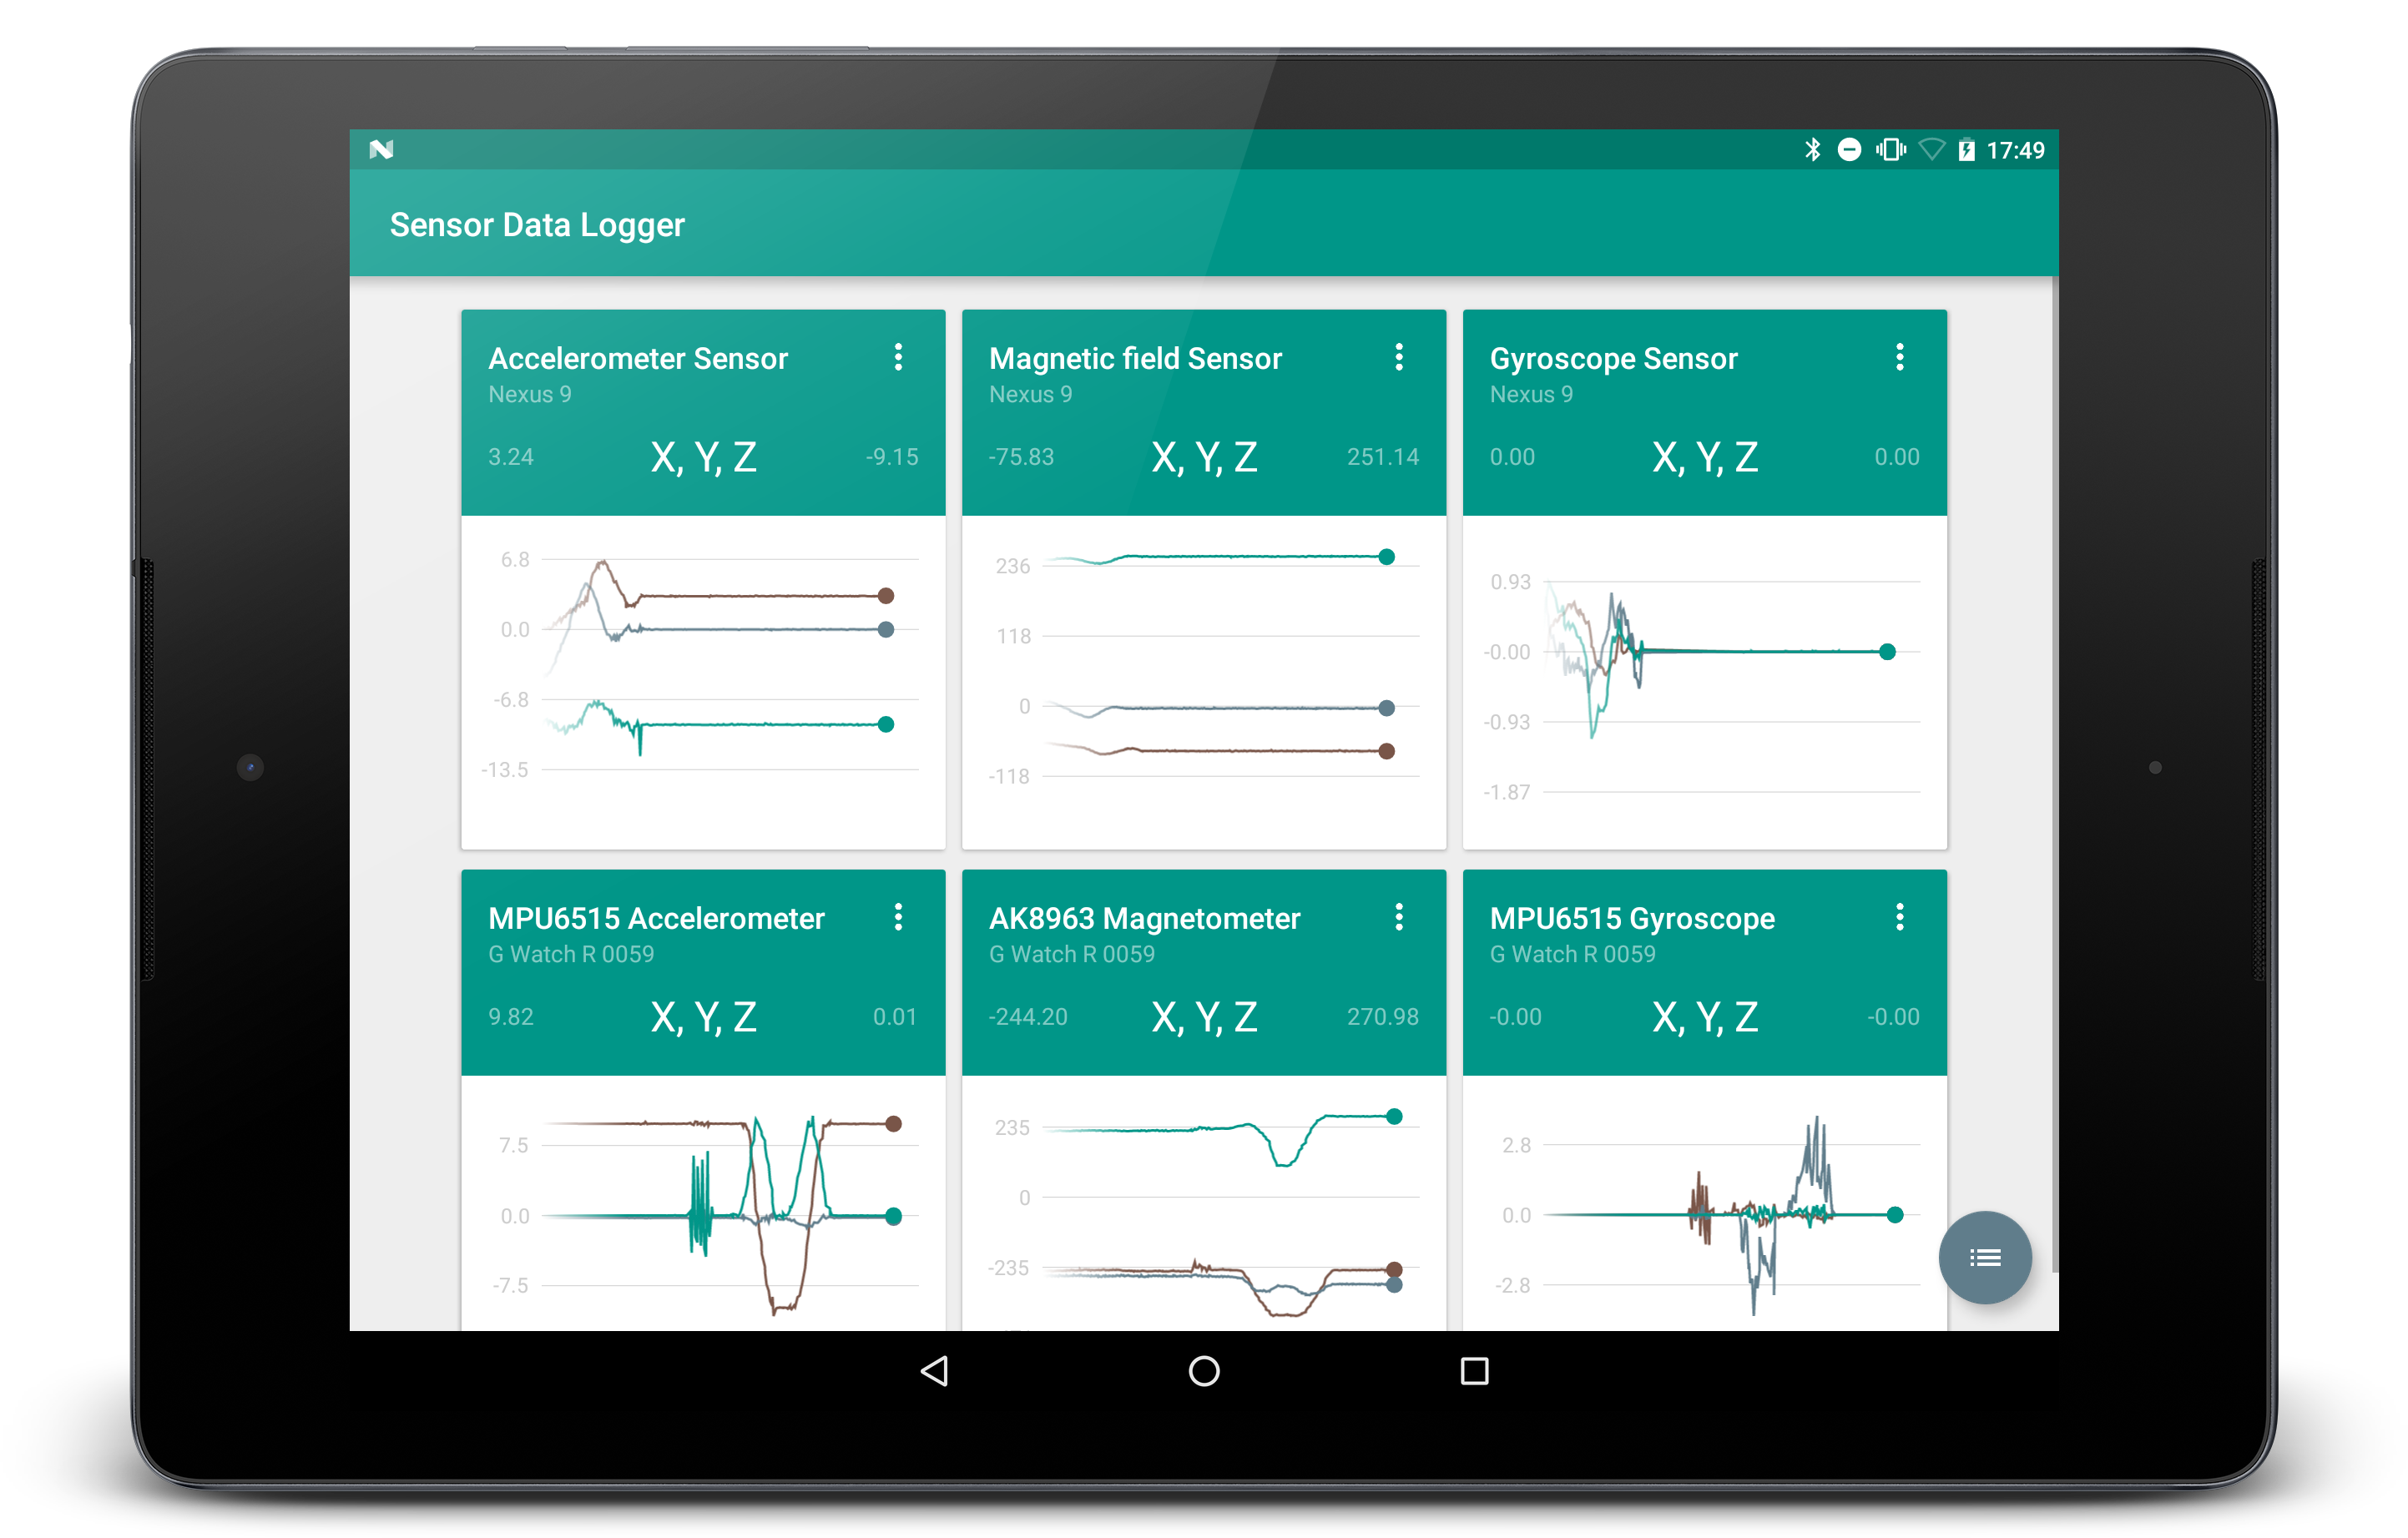
\includegraphics[width=\linewidth]{images/app/charts_landscape_framed.png}
	}
	\caption[Caption for Sensor Data Logger App]{Sensor Data Logger App}
	\label{fig:sensorDataLoggerApp}
\end{figure}

Code samples in the following sections are snippets from this project and can be seen in context in the GitHub repository\footnote{\href{https://github.com/Steppschuh/Sensor-Data-Logger}{https://github.com/Steppschuh/Sensor-Data-Logger}}.

\clearpage

\subsection{Accessing Data}

Android provides the |SensorManager|\cite{androiddocs:sensormanager} system service class in order to grant applications access to the device sensors.
The supported sensors can be divided into three categories:

\begin{itemize}[noitemsep]
	\item \textbf{Environmantal sensors} (thermometers, barometers and photometers)
	\item \textbf{Motion sensors} (accelerometers, gyroscopes and gravity sensors)
	\item \textbf{Position sensors} (magnetometers and orientation sensors)
\end{itemize}

Not all sensors are hardware components, the so called ``virtual-'' or ``synthetic sensors'' derive their data from one or more hardware-based sensors.
Examples for these virtual sensors would be the ``Linear Acceleration Sensor'', which computes its data based on the accelerometer and the force of gravity.

All sensors can be accessed through the Android sensor framework, which provides classes and interfaces that can be used to figure out which sensors are available on the current device, which capabilities they have and what data they produce.

\subsubsection{Checking Availability}
While most devices have an accelerometer and a magnetometer, only a few have a thermometer.
The availability of sensors can't be guaranteed, it's good practice to check this at runtime:

\begin{lstlisting}[label=getsensormanager]
// get a SensorManager instance
SensorManager sensorManager = (SensorManager) getSystemService(Context.SENSOR_SERVICE);

// get a list of available sensors
List<Sensor> deviceSensors = sensorManager.getSensorList(Sensor.TYPE_ALL);

// check if an accelerometer is available
Sensor accelerometer = sensorManager.getDefaultSensor(Sensor.TYPE_ACCELEROMETER);
if (accelerometer != null) {
	// use accelerometer
} else {
	// perform error handling
}
\end{lstlisting}

If a sensor is available, public methods from the |Sensor|\cite{androiddocs:sensor} class can be used to get detailed information about it.
The name, vendor, version, data range and reporting delay are useful properties, especially because one device can have multiple sensors of the same type.

\subsubsection{Monitoring data changes}
In order to get access to the actual data, a |SensorEventListener|\cite{androiddocs:sensoreventlistener} needs to be registered at the |SensorManager| instance. The |SensorEventListener| is an interface which exposes two callback methods:

\begin{lstlisting}[label=registersensoreventlistener]
// create a new SensorEventListener
SensorEventListener listener = new SensorEventListener() {
	@Override
	public void onSensorChanged(SensorEvent event) {
		// sensor reported new data
	}

	@Override
	public void onAccuracyChanged(Sensor sensor, int accuracy) {
		// sensor accuracy changed
	}
};

// specify a reporting delay for the sensor
int delay = SensorManager.SENSOR_DELAY_NORMAL;

// register the listener for the accelerometer
sensorManager.registerListener(listener, accelerometer, delay);
\end{lstlisting}

\lipsum[1]
\lipsum[2]
\lipsum[3]
\lipsum[4]
\lipsum[5]
\lipsum[1]
\lipsum[2]
\lipsum[3]
\lipsum[4]
\lipsum[5]

\subsection{Transferring Data}
\begin{itemize}[noitemsep]
	\item What to transfer
		\begin{itemize}
			\item suitable data types
			\item serialization
		\end{itemize}
	\item How to transfer
		\begin{itemize}
			\item Available APIs and Protocols
			\item Pros and cons of different methods
		\end{itemize}
\end{itemize}
\lipsum[1]
\lipsum[2]
\lipsum[3]
\lipsum[4]
\lipsum[5]
\lipsum[1]
\lipsum[2]
\lipsum[3]
\lipsum[4]
\lipsum[5]
\lipsum[2]
\lipsum[3]
\lipsum[4]
\lipsum[5]


\clearpage